\documentclass{article}
\usepackage[utf8]{inputenc}

\title{ML for Dynamic Systems}
\author{Cyprien Neverov}
\date{March 2020}

\usepackage{natbib}
\usepackage{graphicx}

\begin{document}

This short report is a non-exhaustive list of a few ways ML techniques are used to work with dynamical systems. 
The articles mentioned in this document are the ones that were given to me and some that I came across during my two-day bibliographical research. 

\section{Data-driven discretization}

Image processing research has evolved a lot in the past five years. 
Today state of the art techniques are able to perform intelligent tasks on images way better than humans.
One example of such a task is super-resolution, where a model infers an additional set of pixels in order to enhance the overall quality and sharpness of an image.
Similar techniques can be used to refine a simulation discretization and enhance the quality of the numerical solution.
The authors of \cite{Bar-Sinai15344} propose to use neural networks to learn Taylor coefficients to do spatial derivation, which is closely related to interpolating missing values like in super-resolution. 
This allows them to run time integrations on much coarser grids while still preserving the overall quality of the numerical solution.

\begin{quote}
    ... we propose data-driven discretization, a method that uses machine learning to systematically derive discretization for continuous physical systems. On a series of model problems, data-driven discretization gives accurate solutions with a dramatic drop in required resolution.
\end{quote}

The architecture of their models is designed to minimize the error on the few next time steps. 
The model learns on data generated by fine simulations
The authors provide both code to reproduce their results and code to adapt their method to other problems. 


\section{Learning control functions}

One of the most obvious uses of ML in control theory would be to approximate the optimal control function with neural networks.
In the literature there are examples of both supervised learning and reinforcement learning used for this purpose.
For example the authors of \cite{nakamurazimmerer2019adaptive} show that a neural network is able to learn a value function given a set of open-loop examples. 
Which then allows them to deduce the feedback control from the value function.

On the other hand, in \cite{kunisch} the authors introduce the mathematical foundations for training neural networks to do optimal control directly without using precomputed examples.
The method is close to RL (reinforcement learning) because it involves solving HJB equation.
Authors provide a few numerical examples but no code seems to be provided which means that it could be interesting to implement their method.



\section{Identifying systems}

Since neural networks are universal approximators they can be used to model the behavior of a complex dynamic systems. 
I cases where the system is not well understood, it can be useful to be able to cheaply simulate the dynamics. 
In \cite{long2017pdenet} the authors say that the neural networks are able to mimic dynamic systems for relatively long periods of time and also that it is possible to inspect the NN to deduce derivations and other operations of the underlying PDEs.


\section{Intelligent meshing}

There are also efforts directed towards generating meshes for finite-element methods.
Like for example in \cite{meshing} where the authors use neural networks for this purpose.

\begin{figure}[h]
\caption{Example of a neural meshing}
\centering
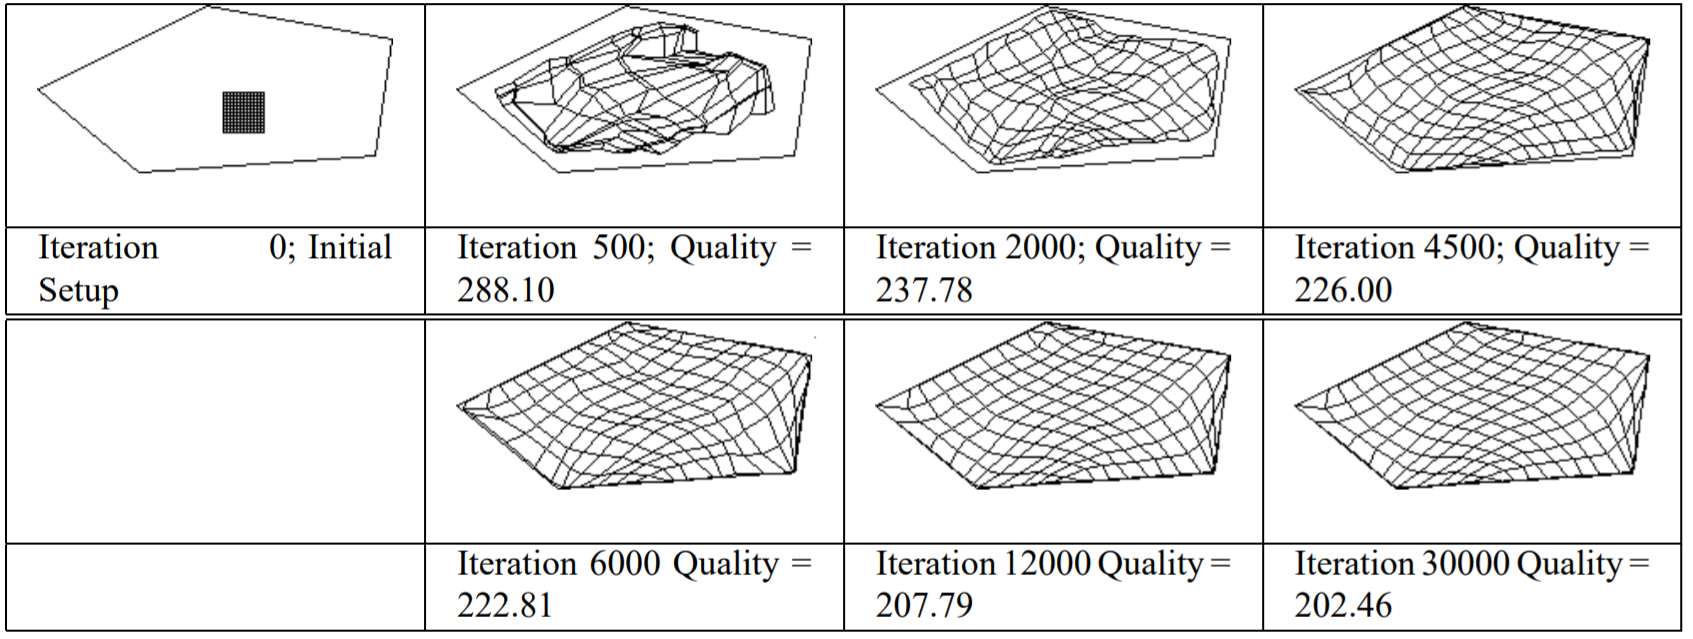
\includegraphics[width=0.5\textwidth]{meshing}
\end{figure}

The article uses self-organizing neural networks which apparently were introduced back in the late 80s in \cite{kohonen2012self}.

To the best of my knowledge they have very little to do with actual neural networks.
Which leaves room to try deep neural networks at this task.

\section{Additional resources}

It is worth mentioning that there is a book \cite{brunton2019data} by S. Brunton and J. Kutz called \textit{Data-driven science and engineering: Machine learning, dynamical systems, and control} that was recently published. 
It's name and description suggests that it is very closely related to the problems we are interested in.
However, it is also stated that it is ``primarily to educate our advanced undergrad and beginning graduate students from engineering and physical science departments.'' Which means that it is probably more oriented towards explaining well established techniques.


\bibliographystyle{plain}
\bibliography{references}
\end{document}
